\documentclass[10pt]{article}
\usepackage[polish]{babel}
\usepackage[utf8]{inputenc}
\usepackage[T1]{fontenc}
\usepackage{amsmath}
\usepackage{amsfonts}
\usepackage{amssymb}
\usepackage[version=4]{mhchem}
\usepackage{stmaryrd}
\usepackage{graphicx}
\usepackage[export]{adjustbox}
\graphicspath{ {./images/} }

\title{GIMNAZJUM }

\author{}
\date{}


\newcommand\Varangle{\mathop{{<\!\!\!\!\!\text{\small)}}\:}\nolimits}

\begin{document}
\maketitle
\begin{enumerate}
  \item Na bokach \(B C\) i \(C D\) kwadratu \(A B C D\) wybrano odpowiednio takie punkty \(P\) i \(Q\), że \(B P+D Q=P Q\). Wykazać, że środek okręgu opisanego na trójkącie \(A P Q\) leży na przekątnej \(A C\) kwadratu \(A B C D\).
  \item Na bokach \(B C\) i \(C D\) równoległoboku \(A B C D\) zbudowano kwadraty \(C D E F\) i \(B C G H\). Udowodnij, że \(|A C|=|F G|\).
  \item Udowodnij, że jeżeli \(a \neq b\) i \(a+b=2 c\), to\\
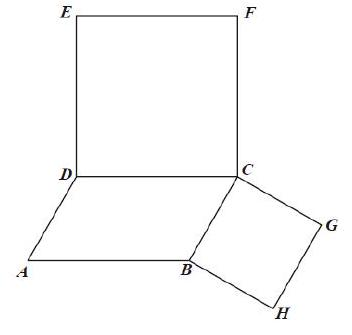
\includegraphics[max width=\textwidth, center]{2024_11_21_f2eb1b7285ec9169cbc0g-1}
\end{enumerate}

\[
\frac{a}{a-c}+\frac{b}{b-c}=2
\]

\section*{LICEUM}
\begin{enumerate}
  \item Dany jest trójkąt \(A B C\), w którym \(\Varangle A C B=60^{\circ}\) oraz \(A C<B C\). Punkt \(D\) leży na boku \(B C\), przy czym \(B D=A C\). Punkt \(E\) jest punktem symetrycznym do punktu \(A\) względem punktu \(C\). Udowodnić, że \(A B=D E\).\\
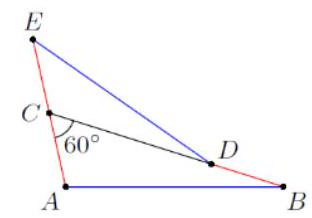
\includegraphics[max width=\textwidth, center]{2024_11_21_f2eb1b7285ec9169cbc0g-1(1)}
  \item Punkt \(S\) jest środkiem ciężkości trójkąta \(A B C\), punkty \(A_{1}, B_{1}, C_{1}\) są odpowiednio środkami boków \(B C, A C, A B\), zaś punkty \(K, L, M\) - środkami odcinków \(S A, S B, S C\). Wykaż, że \(\Delta A_{1} B_{1} C_{1} \equiv \Delta K L M\).
  \item Przez \([x]\) oznaczamy największą liczbę całkowitą nie większą od \(x\). Udowodnij, że dla każdej liczby naturalnej \(n\)\\
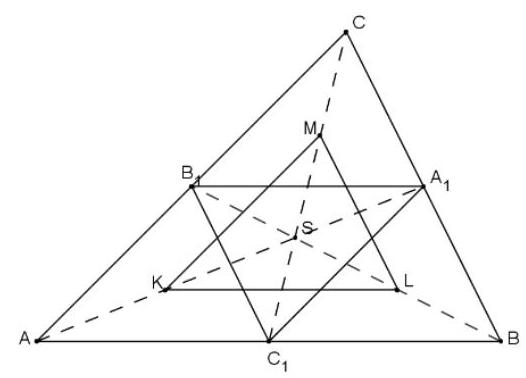
\includegraphics[max width=\textwidth, center]{2024_11_21_f2eb1b7285ec9169cbc0g-1(2)}\\
liczba
\end{enumerate}

\[
\left[\frac{n+4}{2}\right]+3 n-2 \cdot(-1)^{n}
\]

jest podzielna przez 7.


\end{document}